\documentclass[11pt]{article}

\usepackage[a4paper,margin=1in]{geometry}
\usepackage[T1]{fontenc}
\usepackage[utf8]{inputenc}
\usepackage{lmodern}
\usepackage{microtype}
\usepackage{amsmath,amssymb,amsthm,mathtools}
\usepackage{bm}
\usepackage{graphicx}
\usepackage{booktabs}
\usepackage{enumitem}
\usepackage{xcolor}
\usepackage{hyperref}
\usepackage[nameinlink,capitalise,noabbrev]{cleveref}

\hypersetup{
  colorlinks=true,
  linkcolor=blue!60!black,
  citecolor=blue!60!black,
  urlcolor=blue!60!black,
  pdftitle={Higher-Order Jet Cancellation for Anchored Divided-Difference Iterations},
  pdfauthor={Ivan Besevic}
}

\newtheorem{theorem}{Theorem}[section]
\newtheorem{proposition}[theorem]{Proposition}
\newtheorem{corollary}[theorem]{Corollary}
\theoremstyle{definition}
\newtheorem{definition}[theorem]{Definition}
\newtheorem{remark}[theorem]{Remark}
\newtheorem{example}[theorem]{Example}

\newcommand{\C}{\mathbb{C}}
\newcommand{\R}{\mathbb{R}}
\newcommand{\Oterm}{\mathcal{O}}
\newcommand{\dd}{\,\mathrm{d}}
\newcommand{\Fphi}{F_{\phi}}
\newcommand{\PFa}{P_{F,a}}
\newcommand{\Pphia}{P_{\phi,a}}
\newcommand{\ord}{\operatorname{ord}}
\newcommand{\jet}{\operatorname{jet}}

\title{Higher-Order Jet Cancellation for Anchored Divided-Difference Iterations\\
\large Inverse-Jet Charts, Residual Order Ladders, and Geometric Preconditioning}
\author{Ivan Besevic\\Independent Mathematical Research\\\texttt{github.com/ivan-fr/poussiere\_de\_x}}
\date{May 2026}

\begin{document}
\maketitle

\begin{abstract}
The anchored divided-difference map
\[
P_{F,a}(s)=a-\frac{F(a)}{F[a,s]},
\qquad
F[a,s]=\frac{F(a)-F(s)}{a-s},
\]
turns every simple zero of $F$ into a fixed point whose local multiplier is governed by the first nonlinear terms of $F$ at the root. Earlier chart optimization cancels the quadratic defect of $F_{\phi}=G\circ\phi$ by imposing $F''_{\phi}(r)=0$. This paper develops the higher-order version. A chart is called $m$-flat at a simple root if, in root-normalized coordinates,
\[
G(\phi(s))=s+\Oterm(s^{m+1}).
\]
We prove the residual order ladder: if
\[
F(s)=s+c_{m+1}s^{m+1}+\Oterm(s^{m+2}),
\]
then
\[
P'_{F,a}(0)=c_{m+1}a^m+\Oterm(a^{m+1})
\]
and the two-point error has leading homogeneous term
\[
P_{F,a}(s)=c_{m+1}as(a^{m-1}+a^{m-2}s+\cdots+s^{m-1})+
\Oterm((|a|+|s|)^{m+2}).
\]
Thus fixed-anchor convergence remains linear for a fixed anchor, but its multiplier can be made an arbitrarily high power of the anchor distance by flattening the transformed equation. We then prove that the unique $m$-jet achieving this cancellation is the truncated local inverse of $G$, and we give a practical recurrence for its coefficients. The example $G(z)=e^z-2$ shows, through Python-generated figures, the progression from affine normalization to quadratic, cubic, quartic, and quintic inverse jets. The central message is that higher residual order can be obtained not by changing the anchored iteration, but by changing the local geometry in which the iteration is performed.
\end{abstract}

\paragraph{One-sentence summary.}
Higher-order inverse jets flatten the transformed equation $G\circ\phi$, and an $m$-flat chart changes the anchored residual multiplier from $\Oterm(h)$ to $\Oterm(h^m)$, where $h$ is the anchor distance.

\section{Introduction}
The monomial Pandrosion construction produces a derivative-free fixed-point map whose denominator is the finite geometric sum $S_p(s)=1+s+\cdots+s^{p-1}$. The analytic continuation of that construction replaces the monomial sum by the anchored divided difference $F[a,s]$ and obtains the fixed-anchor secant map
\[
P_{F,a}(s)=a-\frac{F(a)}{F[a,s]}.
\]
At a simple zero $r$, its exact multiplier is
\[
P'_{F,a}(r)=1-\frac{F'(r)}{F[a,r]}.
\]
When the anchor is close to the root, the multiplier has the local expansion
\[
P'_{F,a}(r)=\frac{F''(r)}{2F'(r)}(a-r)+\Oterm((a-r)^2).
\]
The first chart-optimization result says that, after passing to a chart $\phi$, one should cancel $F''_{\phi}(r)$, where $F_{\phi}=G\circ\phi$. That cancellation changes the multiplier from first order in $a-r$ to second order in $a-r$.

This paper asks the next natural question:
\begin{quote}
\emph{Can one cancel not only the quadratic defect, but the entire local nonlinear jet of the transformed equation?}
\end{quote}
The answer is yes, locally and to arbitrary finite order. The optimal $m$-jet is simply the $m$-jet of the local inverse of $G$ at the root value. This observation is conceptually simple but structurally useful: it turns chart selection into a finite-order normal-form problem.

\paragraph{What is new here.}
The paper's contribution is not a new secant formula. The fixed-anchor secant formula is classical. The new structure is the following hierarchy.
\begin{enumerate}[label=(\roman*)]
    \item If $G\circ\phi$ is only root-normalized, the raw multiplier is generally $\Oterm(h)$.
    \item If $G\circ\phi=s+\Oterm(s^3)$, the raw multiplier is $\Oterm(h^2)$.
    \item If $G\circ\phi=s+\Oterm(s^{m+1})$, the raw multiplier is $\Oterm(h^m)$.
    \item The unique $m$-jet realizing this flattening is the truncated inverse jet of $G$.
\end{enumerate}
Thus the iteration is kept fixed while the coordinates are made increasingly linear.

\paragraph{Important limitation.}
For a fixed nonzero anchor, the raw map is still a linearly convergent fixed-point iteration. Higher-order jet cancellation does not magically make a fixed-anchor iteration have order $m+1$ in the current error. Rather, it makes the linear multiplier scale like the $m$-th power of the anchor distance. This distinction is essential.

\section{Anchored maps and residual order}
Let $F$ be analytic near $0$, with a simple zero at $0$ and $F'(0)\neq 0$. After multiplying $F$ by a nonzero constant, we may assume $F'(0)=1$. This normalization does not change the fixed points of the anchored map.

\begin{definition}[Residual order]
Assume
\begin{equation}\label{eq:residual-expansion}
F(s)=s+c_{m+1}s^{m+1}+\Oterm(s^{m+2})
\end{equation}
with $m\geq 1$ and with all coefficients of $s^2,\ldots,s^m$ equal to zero. We say that $F$ is \emph{$m$-flat} at the root. The coefficient $c_{m+1}$ is the first obstruction beyond the identity model.
\end{definition}

For $m=1$, this is just ordinary root normalization: $F(s)=s+c_2s^2+\cdots$. For $m=2$, the quadratic term is cancelled: $F(s)=s+c_3s^3+\cdots$. The previous curvature-cancellation condition is exactly the case $m=2$.

\begin{theorem}[Residual order ladder]\label{thm:residual-ladder}
Let $F$ be $m$-flat at $0$ in the sense of \eqref{eq:residual-expansion}, and let $a$ be a small anchor with $F(a)\neq0$. Then
\begin{equation}\label{eq:lambda-order-m}
P'_{F,a}(0)=c_{m+1}a^m+\Oterm(a^{m+1}).
\end{equation}
More sharply, as $(a,s)\to(0,0)$,
\begin{equation}\label{eq:two-point-homogeneous}
P_{F,a}(s)=c_{m+1}as(a^{m-1}+a^{m-2}s+\cdots+s^{m-1})+
\Oterm((|a|+|s|)^{m+2}).
\end{equation}
In particular, for fixed $a$, the linear multiplier is an $m$-th order quantity in the anchor distance.
\end{theorem}

\begin{proof}
The exact multiplier identity gives
\[
P'_{F,a}(0)=1-\frac{aF'(0)}{F(a)}=1-\frac{a}{F(a)}.
\]
Since
\[
F(a)=a+c_{m+1}a^{m+1}+\Oterm(a^{m+2})
=a\bigl(1+c_{m+1}a^m+\Oterm(a^{m+1})\bigr),
\]
we get
\[
\frac{a}{F(a)}=1-c_{m+1}a^m+\Oterm(a^{m+1}),
\]
which proves \eqref{eq:lambda-order-m}.

For the two-point statement, use the equivalent form
\[
P_{F,a}(s)=s-\frac{F(s)}{F[a,s]}.
\]
From \eqref{eq:residual-expansion},
\[
F[a,s]
=1+c_{m+1}\frac{a^{m+1}-s^{m+1}}{a-s}+\Oterm((|a|+|s|)^{m+1}).
\]
The polynomial quotient is
\[
\frac{a^{m+1}-s^{m+1}}{a-s}=a^m+a^{m-1}s+\cdots+s^m.
\]
Expanding the reciprocal of $F[a,s]$ gives
\[
\frac{1}{F[a,s]}
=1-c_{m+1}(a^m+a^{m-1}s+\cdots+s^m)+\Oterm((|a|+|s|)^{m+1}).
\]
Substitution into $s-F(s)/F[a,s]$ gives
\[
P_{F,a}(s)
=c_{m+1}s(a^m+a^{m-1}s+\cdots+s^m)-c_{m+1}s^{m+1}
+\Oterm((|a|+|s|)^{m+2}),
\]
which is exactly \eqref{eq:two-point-homogeneous}.
\end{proof}

\begin{remark}[The classical product law as $m=1$]
When $m=1$, formula \eqref{eq:two-point-homogeneous} becomes
\[
P_{F,a}(s)=c_2as+\Oterm((|a|+|s|)^3),
\]
which is the fixed-anchor form of the secant product law. Higher-order jet cancellation replaces the bilinear product $as$ by a homogeneous product of degree $m+1$.
\end{remark}

\section{Higher-order chart flattening}
Let $G$ be analytic near a simple zero $\rho$, so $G(\rho)=0$ and $G'(\rho)\neq0$. A chart $\phi$ with $\phi(0)=\rho$ transforms the equation into
\[
F_{\phi}(s)=G(\phi(s)).
\]
We now define the higher-order analogue of root normalization and curvature cancellation.

\begin{definition}[$m$-flat chart]
A local chart $\phi$ is called \emph{$m$-flat at $\rho$} if
\begin{equation}\label{eq:m-flat-chart}
G(\phi(s))=s+\Oterm(s^{m+1})
\end{equation}
near $s=0$. Equivalently,
\[
(G\circ\phi)'(0)=1,
\qquad
(G\circ\phi)^{(j)}(0)=0\quad(2\leq j\leq m).
\]
\end{definition}

Thus a $1$-flat chart is merely root-normalized. A $2$-flat chart is the curvature-balanced chart from the previous paper. A $3$-flat chart cancels the quadratic and cubic defects, and so on.

\begin{corollary}[Multiplier of an $m$-flat chart]\label{cor:m-flat-multiplier}
If $\phi$ is $m$-flat at $\rho$, then the charted anchored map
\[
P_{\phi,a}(s)=a-\frac{G(\phi(a))}{(G\circ\phi)[a,s]}
\]
satisfies
\[
P'_{\phi,a}(0)=\Oterm(a^m).
\]
If the first nonzero defect is
\[
G(\phi(s))=s+c_{m+1}s^{m+1}+\Oterm(s^{m+2}),
\]
then
\[
P'_{\phi,a}(0)=c_{m+1}a^m+\Oterm(a^{m+1}).
\]
\end{corollary}

\begin{proof}
Apply \Cref{thm:residual-ladder} to $F=G\circ\phi$.
\end{proof}

\section{The inverse-jet theorem}
The ideal chart is the local inverse of $G$. Since $G'(\rho)\neq0$, the inverse function theorem gives a local inverse $\Psi$ satisfying
\[
\Psi(0)=\rho,
\qquad
G(\Psi(s))=s.
\]
This exact chart makes the anchored map converge in one step. In practice one may only use a finite jet of $\Psi$. The next theorem shows that this finite inverse jet is the unique local solution of the higher-order cancellation problem.

Write the Taylor expansion of $G$ at $\rho$ as
\begin{equation}\label{eq:G-taylor}
G(\rho+w)=g_1w+g_2w^2+g_3w^3+\cdots,
\qquad
g_j=\frac{G^{(j)}(\rho)}{j!},
\qquad g_1\neq0.
\end{equation}

\begin{theorem}[Inverse-jet construction]\label{thm:inverse-jet}
For every $m\geq1$, there is a unique polynomial jet
\begin{equation}\label{eq:phi-m-jet}
\phi_m(s)=\rho+b_1s+b_2s^2+\cdots+b_ms^m
\end{equation}
such that
\begin{equation}\label{eq:inverse-jet-flatness}
G(\phi_m(s))=s+\Oterm(s^{m+1}).
\end{equation}
The coefficients are determined recursively by
\begin{equation}\label{eq:inverse-recursion-b1}
b_1=\frac{1}{g_1},
\end{equation}
\begin{equation}\label{eq:inverse-recursion-bn}
b_n=-\frac{1}{g_1}
\sum_{q=2}^{n}g_q
\sum_{\substack{j_1+\cdots+j_q=n\\ j_\ell\geq1}}
b_{j_1}\cdots b_{j_q},
\qquad 2\leq n\leq m.
\end{equation}
Moreover, $\phi_m$ is the truncation of the local inverse $\Psi$ through degree $m$.
\end{theorem}

\begin{proof}
Put
\[
B_m(s)=b_1s+\cdots+b_ms^m.
\]
Then
\[
G(\phi_m(s))=\sum_{q\geq1}g_qB_m(s)^q.
\]
The coefficient of $s$ is $g_1b_1$, so the condition that it equal $1$ gives \eqref{eq:inverse-recursion-b1}. For $n\geq2$, the coefficient of $s^n$ is
\[
g_1b_n+
\sum_{q=2}^{n}g_q
\sum_{\substack{j_1+\cdots+j_q=n\\ j_\ell\geq1}}
b_{j_1}\cdots b_{j_q}.
\]
Setting this coefficient equal to $0$ gives \eqref{eq:inverse-recursion-bn}. Since $b_n$ appears linearly with coefficient $g_1\neq0$, the construction is unique at every degree. The local inverse $\Psi$ satisfies $G(\Psi(s))=s$ exactly, so its Taylor coefficients satisfy the same recursion. Hence $\phi_m$ is precisely its degree-$m$ truncation.
\end{proof}

The first few coefficients are often useful:
\begin{align}\label{eq:first-coefficients}
 b_1&=\frac{1}{g_1},\\
 b_2&=-\frac{g_2}{g_1^3},\\
 b_3&=\frac{2g_2^2}{g_1^5}-\frac{g_3}{g_1^4},\\
 b_4&=-\frac{5g_2^3}{g_1^7}+\frac{5g_2g_3}{g_1^6}-\frac{g_4}{g_1^5}.
\end{align}
In derivative notation,
\begin{equation}\label{eq:derivative-b2-b3}
 b_2=-\frac{G''(\rho)}{2G'(\rho)^3},
\qquad
 b_3=\frac{3G''(\rho)^2-G'(\rho)G'''(\rho)}{6G'(\rho)^5}.
\end{equation}
The coefficient $b_2$ is exactly the quadratic curvature-cancellation coefficient.

\begin{corollary}[Leading defect of a truncated inverse]\label{cor:trunc-defect}
Let $\Psi(s)=\rho+\sum_{j\geq1}b_js^j$ be the local inverse of $G$, and let $\phi_m$ be its degree-$m$ truncation. Then
\begin{equation}\label{eq:trunc-leading-defect}
G(\phi_m(s))=s-g_1b_{m+1}s^{m+1}+\Oterm(s^{m+2}).
\end{equation}
Consequently
\begin{equation}\label{eq:trunc-multiplier}
P'_{\phi_m,a}(0)=-g_1b_{m+1}a^m+\Oterm(a^{m+1}).
\end{equation}
\end{corollary}

\begin{proof}
Write $\phi_m(s)=\Psi(s)-b_{m+1}s^{m+1}+\Oterm(s^{m+2})$. Since $G(\Psi(s))=s$ and $G'(\Psi(s))=g_1+\Oterm(s)$, Taylor expansion in the outer variable gives
\[
G(\phi_m(s))=G(\Psi(s))-g_1b_{m+1}s^{m+1}+\Oterm(s^{m+2}),
\]
which proves \eqref{eq:trunc-leading-defect}. Formula \eqref{eq:trunc-multiplier} follows from \Cref{thm:residual-ladder}.
\end{proof}

\begin{theorem}[Exact inverse chart]\label{thm:exact-inverse}
Let $\Psi$ be the local inverse of $G$ at the simple zero $\rho$, and set $\phi_*(s)=\Psi(s)$. Then $G(\phi_*(s))=s$ exactly, and therefore
\[
P_{\phi_*,a}(s)=0
\]
for every nearby anchor $a$ and every nearby current point $s$ for which the formula is defined. The exact inverse chart gives one-step convergence.
\end{theorem}

\begin{proof}
If $F_{\phi_*}(s)=s$, then $F_{\phi_*}[a,s]=1$ and $F_{\phi_*}(a)=a$. Hence $P_{\phi_*,a}(s)=a-a=0$.
\end{proof}

\section{Uniform local palette consequence}
The original monomial paper used scale palettes, while the general analytic paper used anchor palettes. Higher-order jet cancellation gives a sharper local palette statement.

\begin{proposition}[Higher-order local anchor covering]\label{prop:palette}
Let $K\subset\C$ be compact, and suppose that $G$ has only simple zeros in a neighborhood of $K$. Fix $m\geq1$. Assume that around each zero $\rho_j\in K$ one has chosen an $m$-flat chart $\phi_j$ with uniform bounds on the relevant Taylor remainders. Then there are constants $C>0$ and $h_0>0$ such that, whenever the chart coordinate anchor $a$ satisfies $0<|a|\leq h_0$, the corresponding charted anchored multiplier obeys
\[
|P'_{\phi_j,a}(0)|\leq C|a|^m.
\]
Consequently, a local anchor palette with mesh $h$ has worst local raw multiplier $\Oterm(h^m)$ in $m$-flat coordinates.
\end{proposition}

\begin{proof}
For each chosen chart, \Cref{cor:m-flat-multiplier} gives $P'_{\phi_j,a}(0)=\Oterm(a^m)$. Since the set of roots in $K$ is finite and the Taylor remainder bounds are assumed uniform, the constants may be chosen uniformly after shrinking the neighborhoods if necessary.
\end{proof}

\section{Example: \texorpdfstring{$G(z)=e^z-2$}{G(z)=exp(z)-2}}
Let
\[
G(z)=e^z-2,
\qquad
\rho=\log 2.
\]
The exact local inverse is explicit:
\[
\Psi(s)=\log(2+s)=\rho+\log\left(1+\frac{s}{2}\right).
\]
Thus
\begin{equation}\label{eq:exp-inverse-series}
\Psi(s)=\rho+\sum_{j\geq1}\frac{(-1)^{j+1}}{j2^j}s^j.
\end{equation}
The degree-$m$ inverse jet is
\begin{equation}\label{eq:exp-phim}
\phi_m(s)=\rho+\sum_{j=1}^{m}\frac{(-1)^{j+1}}{j2^j}s^j.
\end{equation}
By \Cref{cor:trunc-defect},
\begin{equation}\label{eq:exp-defect-coef}
G(\phi_m(s))=s+c_{m+1}s^{m+1}+\Oterm(s^{m+2}),
\qquad
c_{m+1}=\frac{(-1)^{m+1}}{(m+1)2^m}.
\end{equation}
Therefore
\begin{equation}\label{eq:exp-lambda-asymptotic}
P'_{\phi_m,a}(0)=\frac{(-1)^{m+1}}{(m+1)2^m}a^m+\Oterm(a^{m+1}).
\end{equation}

\begin{figure}[htbp]
    \centering
    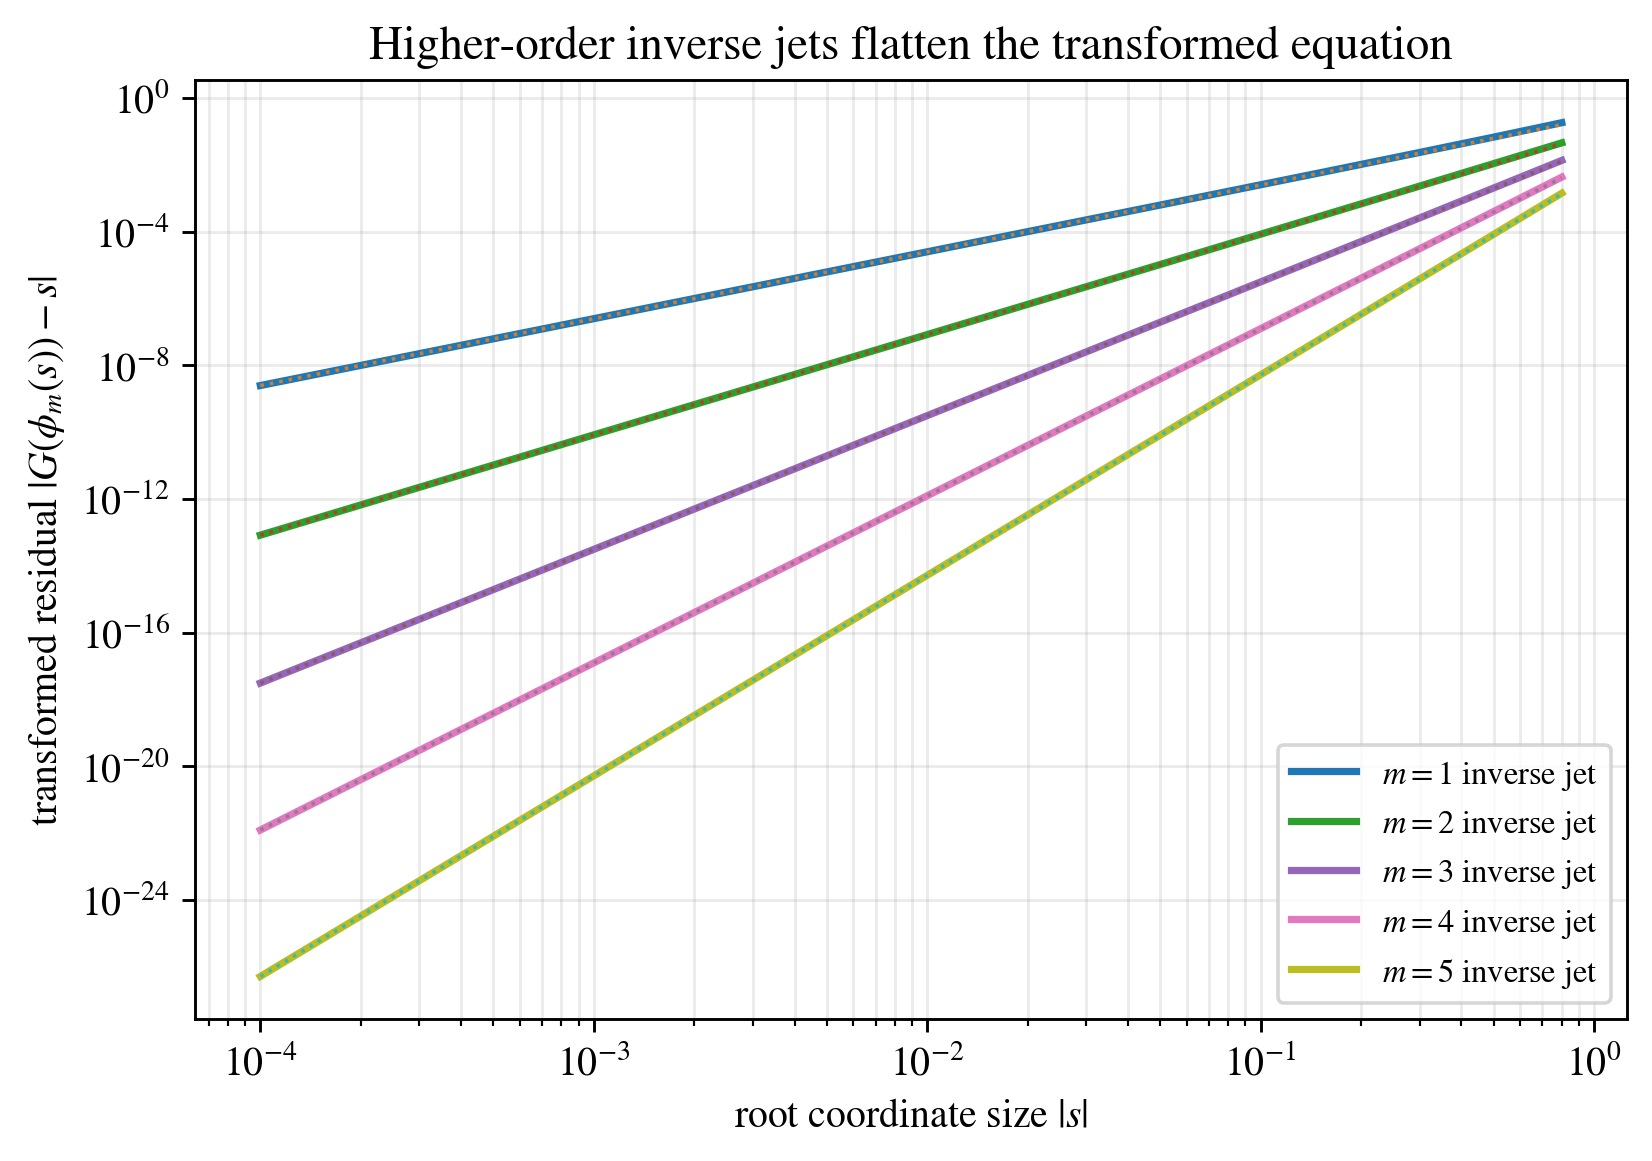
\includegraphics[width=.82\textwidth]{../figures/fig_residual_order_ladder.png}
    \caption{Residual order ladder for $G(z)=e^z-2$. The $m$-th inverse jet makes $G(\phi_m(s))-s$ vanish to order $m+1$. Dotted curves show the leading asymptotic terms from \eqref{eq:exp-defect-coef}.}
    \label{fig:residual-ladder}
\end{figure}

\begin{figure}[htbp]
    \centering
    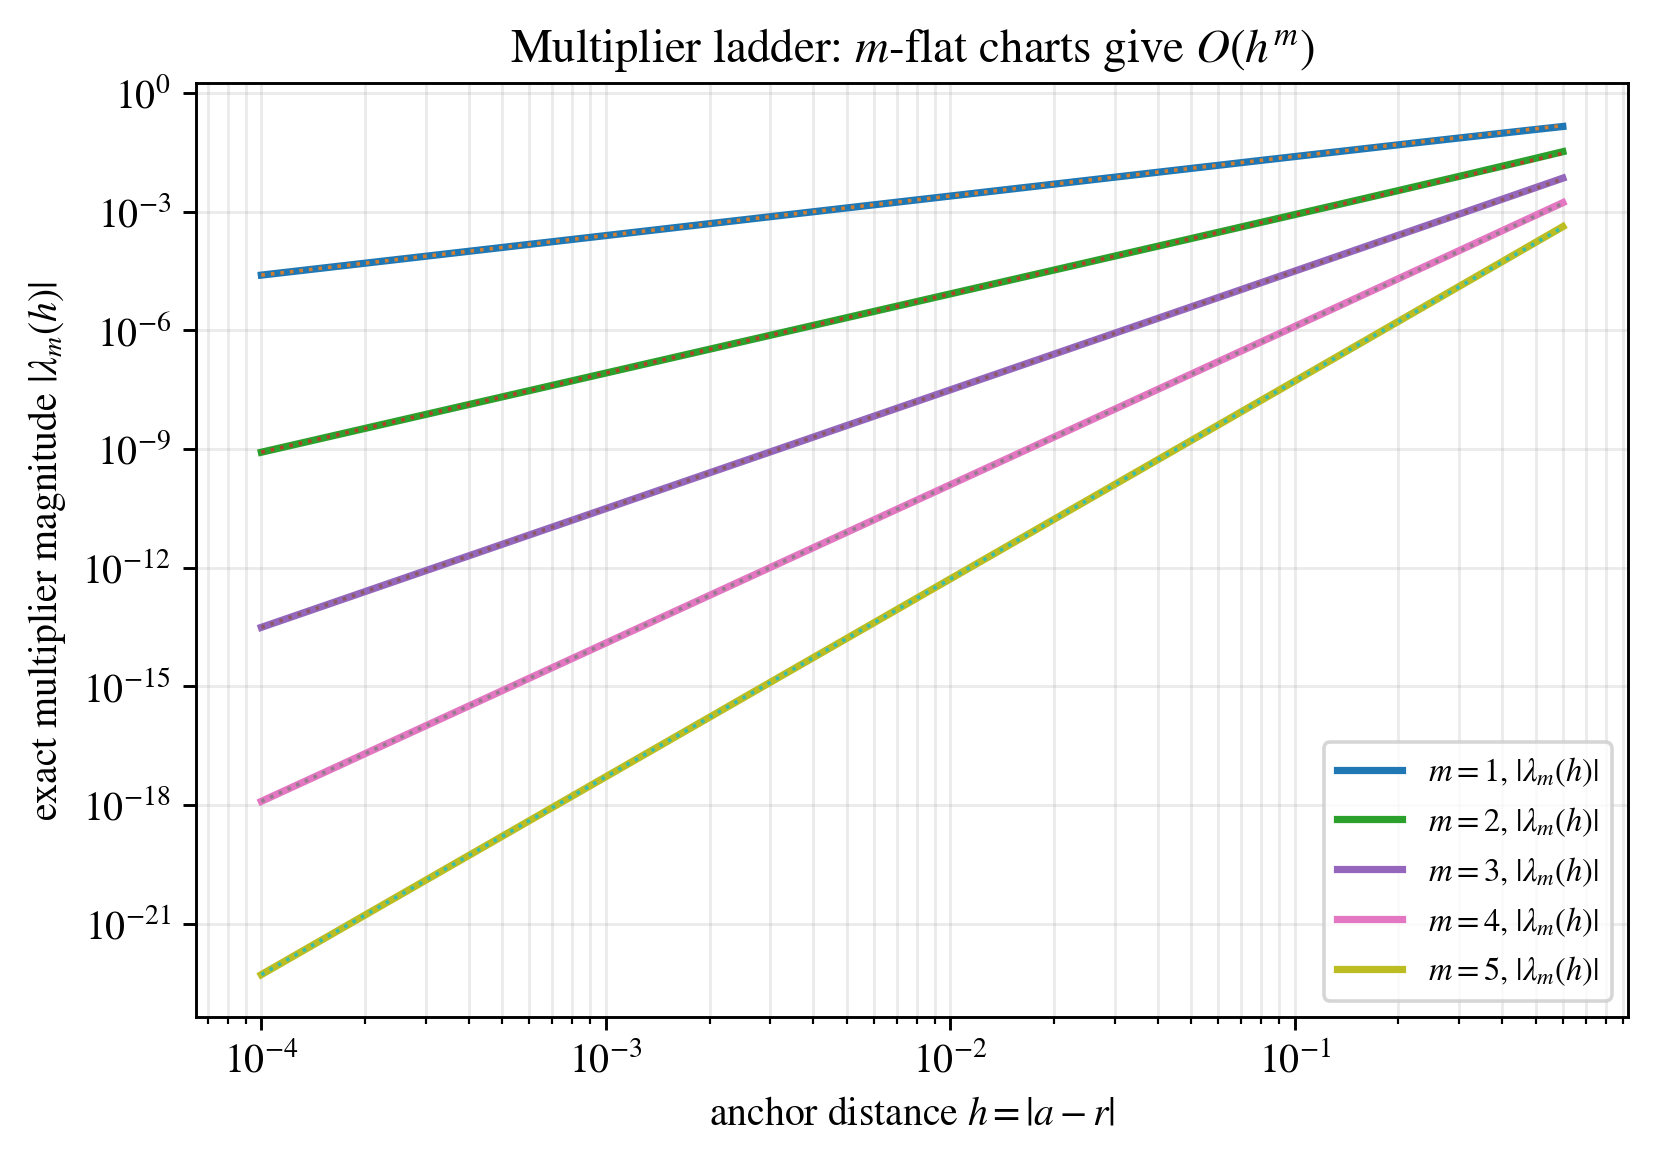
\includegraphics[width=.82\textwidth]{../figures/fig_multiplier_order_ladder.png}
    \caption{Exact multiplier magnitude versus anchor distance. The slope of each curve is $m$ on a log-log scale, confirming $|P'_{\phi_m,a}(0)|=\Oterm(|a|^m)$.}
    \label{fig:multiplier-ladder}
\end{figure}

\begin{figure}[htbp]
    \centering
    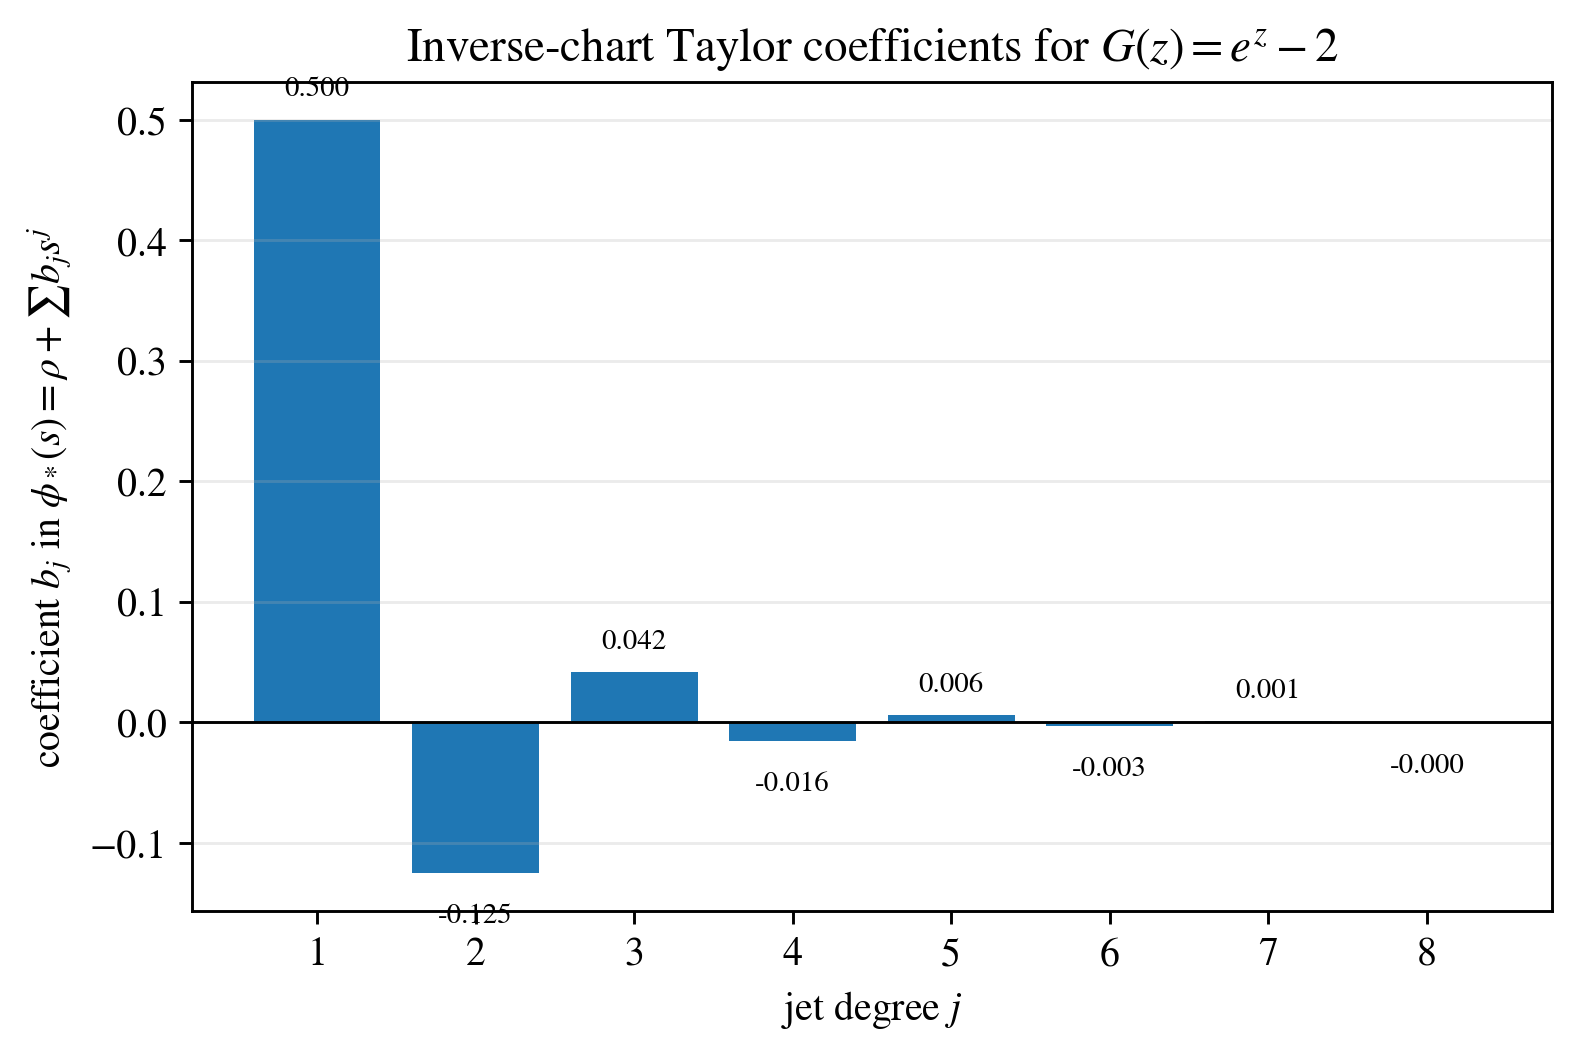
\includegraphics[width=.74\textwidth]{../figures/fig_inverse_jet_coefficients.png}
    \caption{The first inverse-jet coefficients for $G(z)=e^z-2$. These coefficients are the Taylor coefficients of $\log(2+s)$ around $s=0$.}
    \label{fig:jet-coefficients}
\end{figure}

For a concrete fixed-anchor comparison, take $a=0.3$ and $s_0=0.6$ in the chart coordinate. The stopping rule is $|s_n|\leq10^{-12}$. The exact inverse chart reaches the root in one step, while finite jets show the predicted multiplier ladder.

\begin{table}[htbp]
\centering
\begin{tabular}{cccc}
\toprule
jet order $m$ & leading coefficient $c_{m+1}$ & $|P'_{\phi_m,0.3}(0)|$ & iterations \\
\midrule
1 & $1/4$ & $7.3126\times10^{-2}$ & 11 \\
2 & $-1/12$ & $7.8149\times10^{-3}$ & 6 \\
3 & $1/32$ & $8.6607\times10^{-4}$ & 5 \\
4 & $-1/80$ & $1.0355\times10^{-4}$ & 4 \\
5 & $1/192$ & $1.2900\times10^{-5}$ & 3 \\
exact inverse & $0$ & $0$ & 1 \\
\bottomrule
\end{tabular}
\caption{Fixed-anchor comparison for $G(z)=e^z-2$, anchor $a=0.3$, and start $s_0=0.6$. The finite jets do not change the fact that the raw fixed-anchor map is linear for fixed $a$, but they reduce the multiplier by successive powers of $a$.}
\label{tab:example-counts}
\end{table}

\begin{figure}[htbp]
    \centering
    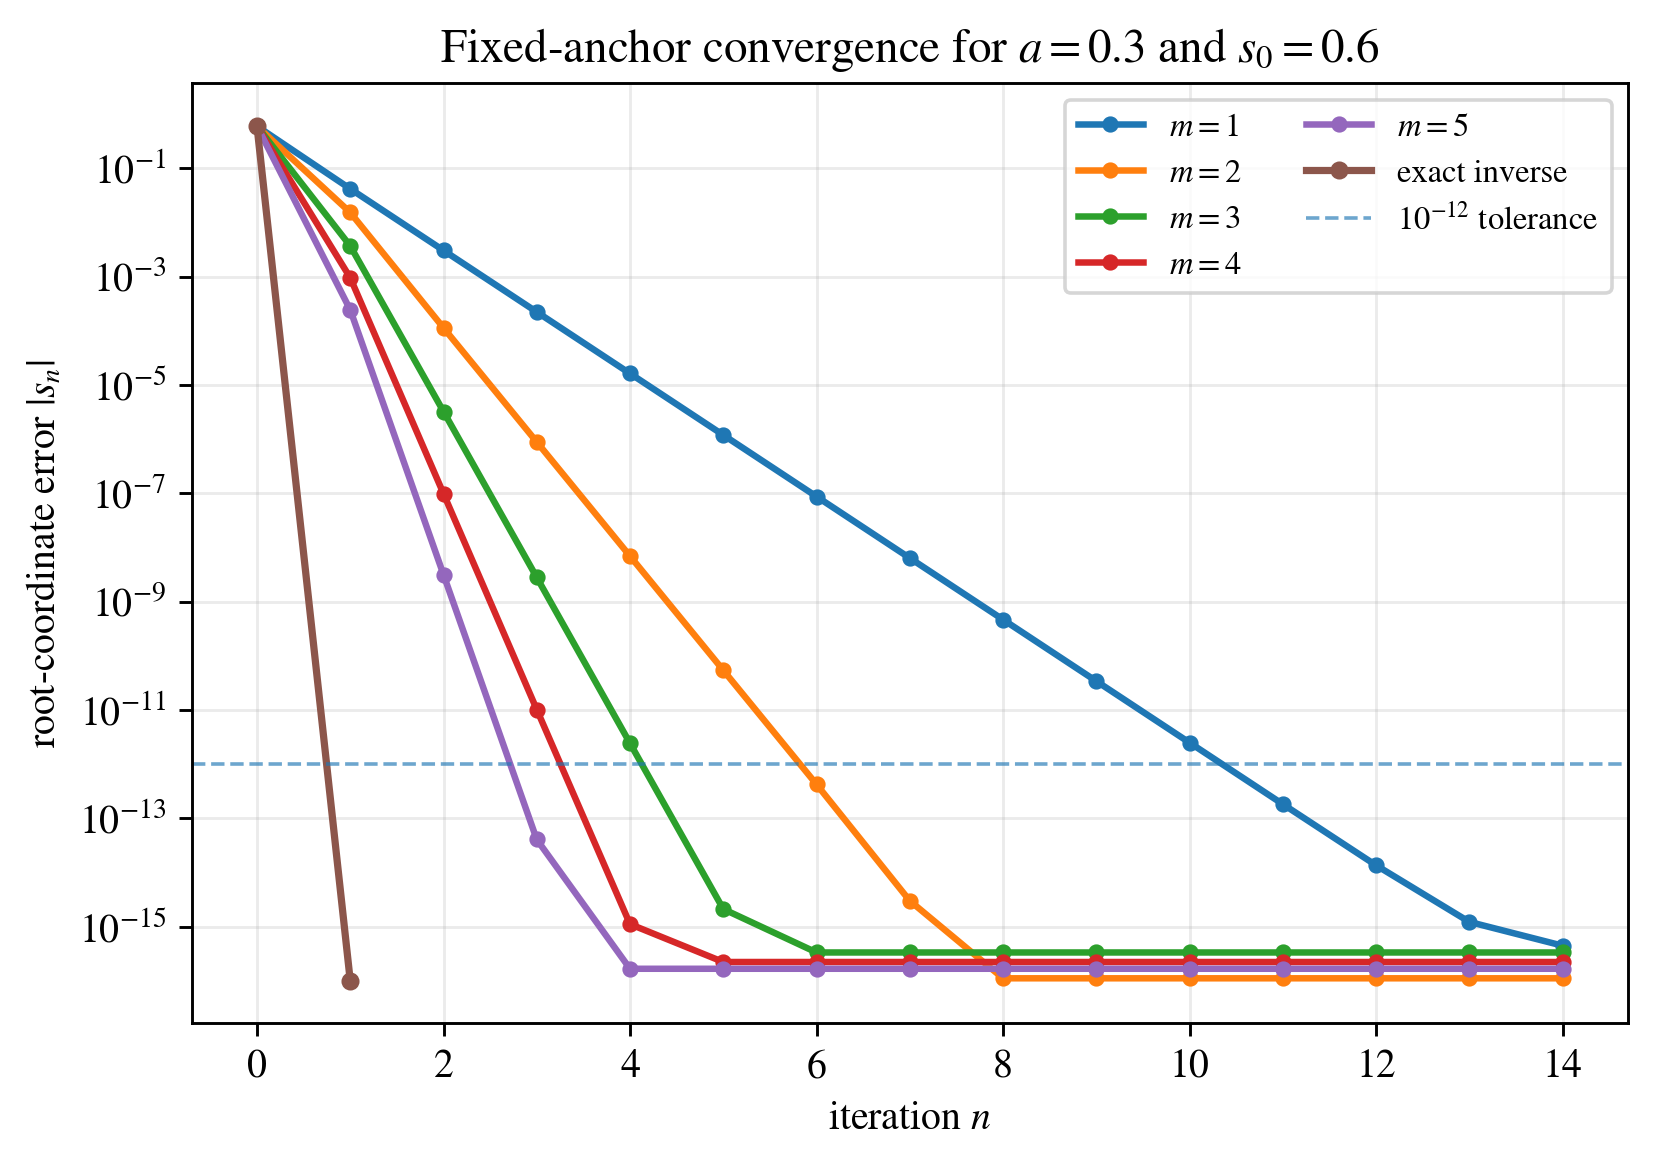
\includegraphics[width=.82\textwidth]{../figures/fig_iteration_histories.png}
    \caption{Error histories for the same test problem. Increasing the inverse-jet order shortens the linear regime; the exact inverse chart collapses the local equation to $F(s)=s$ and therefore reaches the root in one step.}
    \label{fig:iteration-histories}
\end{figure}

\begin{figure}[htbp]
    \centering
    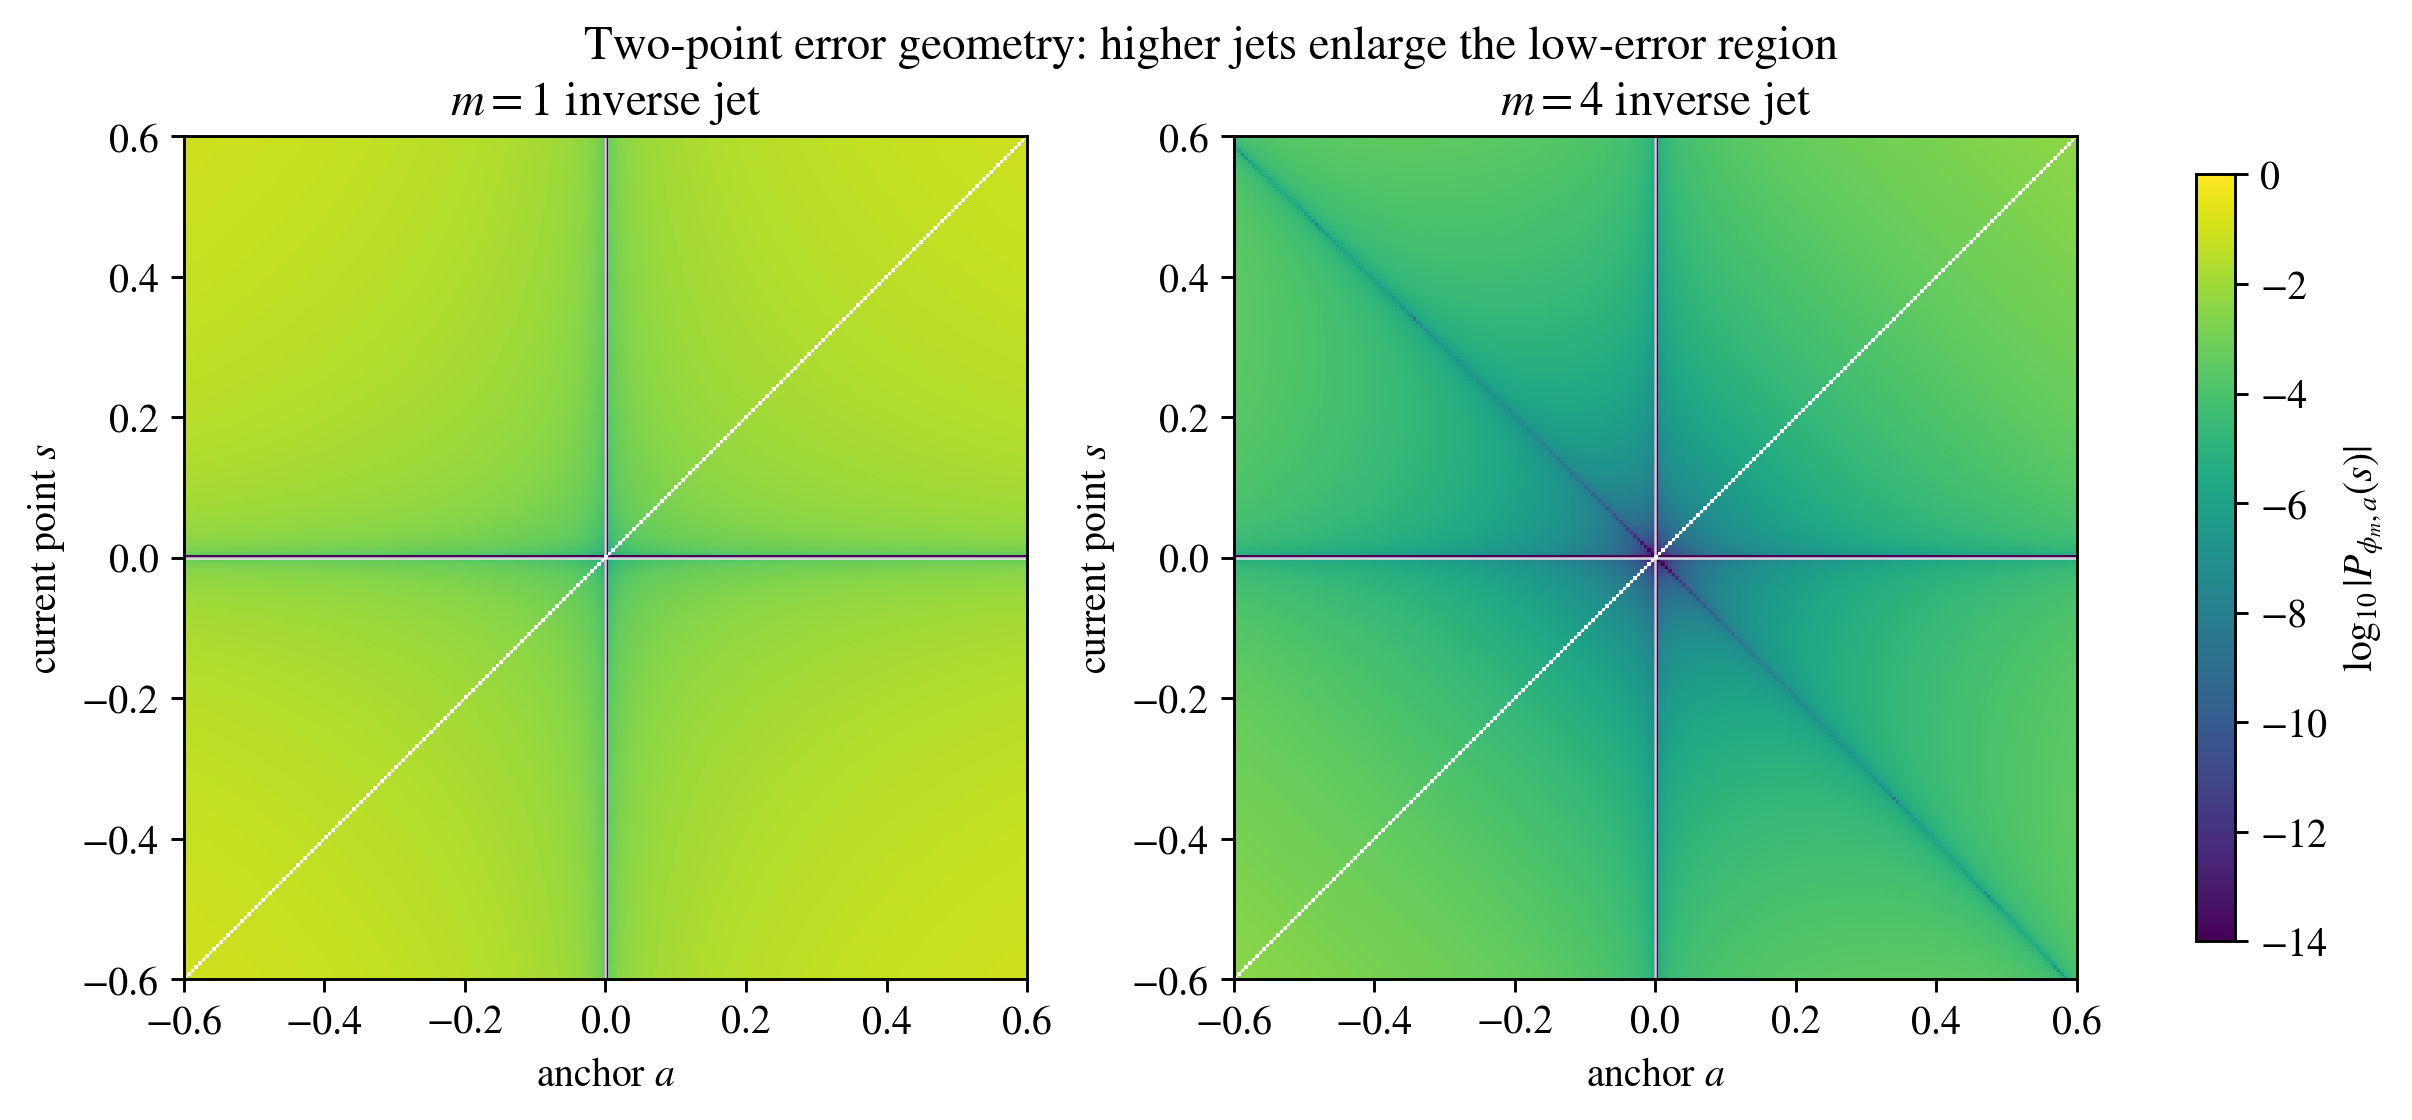
\includegraphics[width=.95\textwidth]{../figures/fig_two_point_error_heatmap.png}
    \caption{Two-point error geometry for $m=1$ and $m=4$. The darker region marks smaller values of $|P_{\phi_m,a}(s)|$. Higher-order jet cancellation enlarges the low-error region around the coordinate axes $a=0$ and $s=0$, in agreement with the homogeneous product law \eqref{eq:two-point-homogeneous}.}
    \label{fig:two-point-heatmap}
\end{figure}

\section{Discussion}
The higher-order inverse-jet construction gives a clean geometric hierarchy:
\begin{center}
\begin{tabular}{lll}
\toprule
chart type & transformed equation & multiplier size \\
\midrule
affine/root-normalized & $s+\Oterm(s^2)$ & $\Oterm(h)$ \\
curvature-balanced & $s+\Oterm(s^3)$ & $\Oterm(h^2)$ \\
$m$-flat inverse jet & $s+\Oterm(s^{m+1})$ & $\Oterm(h^m)$ \\
exact inverse chart & $s$ & $0$ \\
\bottomrule
\end{tabular}
\end{center}
where $h=|a|$ is the anchor distance in the root coordinate.

This hierarchy reframes chart scaling as finite-order normal-form theory. Instead of asking only how to place the root near the anchor, one also asks how to make the transformed equation locally linear. The exact inverse chart is the ideal object, while its finite jets are computable preconditioners.

Several continuations are natural.
\begin{enumerate}[label=(\roman*)]
    \item \textbf{Adaptive inverse jets.} In practice the true root and derivatives may be estimated during iteration. One can update the inverse jet as more information becomes available.
    \item \textbf{Rational inverse approximants.} Pad\'e or rational approximations to the local inverse may enlarge the useful domain beyond the Taylor radius of a polynomial jet.
    \item \textbf{Several variables.} For $G:\C^n\to\C^n$, the analogue of $F''_{\phi}=0$ is cancellation of the quadratic tensor of $G\circ\phi$. Higher-order versions would cancel symmetric multilinear tensors degree by degree.
    \item \textbf{Complex dynamics.} Higher-order flat charts should alter local basins around roots while leaving the global equal-value pole geometry visible.
\end{enumerate}

\section{Conclusion}
Anchored divided-difference iteration has an exact local residual identity. The present paper shows that this identity can be organized into a higher-order chart theory. If the transformed equation is flattened to
\[
G(\phi(s))=s+\Oterm(s^{m+1}),
\]
then the raw anchored multiplier is $\Oterm(h^m)$ in the anchor distance. The unique finite jet that achieves this flattening is the truncated local inverse of $G$.

The conceptual message is therefore simple: the anchored iteration need not be changed in order to obtain a higher-order residual factor in the anchor distance. One may instead change the geometry of the local coordinate. Inverse jets are the finite-order tools that implement this geometric preconditioning.

\section*{Acknowledgments}
The figures in this manuscript were generated with Python and Matplotlib and incorporated into the final manuscript with \LaTeX. This draft is intended as a mathematical continuation of the monomial Pandrosion, general anchored divided-difference, and optimal-chart manuscripts.

\begin{thebibliography}{10}

\bibitem{BesevicMonomial}
I.~Besevic,
\newblock \emph{A Monomial Pandrosion Scheme: Contraction, Chart Scaling, and Steffensen Acceleration for $z^p=x$},
\newblock Independent Mathematical Research, manuscript, May 2026.

\bibitem{BesevicAnchored}
I.~Besevic,
\newblock \emph{Anchored Pandrosion for General Analytic Equations: Divided-Difference Fixed Points, Chart Selection, and Steffensen Acceleration},
\newblock Independent Mathematical Research, manuscript, May 2026.

\bibitem{BesevicOptimalCharts}
I.~Besevic,
\newblock \emph{Optimal Geometric Charts for Anchored Divided-Difference Iterations: Local Linearization, Curvature Cancellation, and Jet-Optimal Preconditioning},
\newblock Independent Mathematical Research, manuscript, May 2026.

\bibitem{Aitken}
A.~C. Aitken,
\newblock On Bernoulli's numerical solution of algebraic equations,
\newblock \emph{Proceedings of the Royal Society of Edinburgh} \textbf{46} (1926), 289--305.

\bibitem{Steffensen}
J.~F. Steffensen,
\newblock Remarks on iteration,
\newblock \emph{Skandinavisk Aktuarietidskrift} \textbf{16} (1933), 64--72.

\bibitem{Traub}
J.~F. Traub,
\newblock \emph{Iterative Methods for the Solution of Equations},
\newblock Prentice--Hall, 1964.

\bibitem{Householder}
A.~S. Householder,
\newblock \emph{The Numerical Treatment of a Single Nonlinear Equation},
\newblock McGraw--Hill, 1970.

\bibitem{OrtegaRheinboldt}
J.~M. Ortega and W.~C. Rheinboldt,
\newblock \emph{Iterative Solution of Nonlinear Equations in Several Variables},
\newblock Academic Press, 1970.

\bibitem{Henrici}
P.~Henrici,
\newblock \emph{Applied and Computational Complex Analysis},
\newblock Wiley, 1974--1986.

\end{thebibliography}

\end{document}
